\documentclass[a4paper]{article}
\usepackage[left=3.18cm,right=3.18cm,top=2.54cm,bottom=2.54cm]{geometry}
\usepackage{CJK}
\usepackage{indentfirst}
\usepackage{amsmath}
\usepackage{graphicx}
\usepackage{booktabs}
%\usepackage{epstopdf}
%\usepackage{epsf}

%%%%%%%%
%%%%%%%%
\usepackage{listings}
\begin{CJK}{UTF8}{gbsn}
\usepackage[usenames,dvipsnames,svgnames,table]{xcolor} % 用于code
\lstset{
	basicstyle=\ttfamily,
	xleftmargin=2pc, % 整体布局
	xrightmargin=2pc,
	backgroundcolor=\color{Lavender}, % 背景色
	rulecolor=\color{Silver}, % 边框颜色
	frame=single,% 边框
	commentstyle=\ttfamily\color{green!40!black},
	texcl=true,
}
\lstdefinelanguage{SAC} {
	keywords={SAC>}, % SAC提示符
	otherkeywords={SAC>}, % SAC提示符
	sensitive=true,
	comment=[l][{\color{green!40!black}}]{\#},
}
\lstnewenvironment{SACCode}{
	\lstset{
		language={SAC}, % 语言
		keywordstyle=\color{blue!70}\bfseries, % 关键字颜色
	}
}{}
\lstdefinelanguage{bash} {
	keywords={bash>}, % bash提示符
	otherkeywords={bash>}, % bash提示符
	sensitive=true,
	comment=[l][{\color{green!40!black}}]{\#},
}
\lstnewenvironment{bashCode}{
	\lstset{
		language={bash}, % 语言
		keywordstyle=\color{blue}, % 关键字颜色
	}
}{}
\lstdefinelanguage{file} {
	keywords={\#}, % 注释提示符
	otherkeywords={\#}, % 注释提示符
	sensitive=true,
	comment=[l][{\color{green!40!black}}]{\#},
}
\lstnewenvironment{fileCode}{
	\lstset{
		backgroundcolor=\color{green!20!white}, % 背景色
		language={file}, % 语言
		keywordstyle=\color{green!40!black}, % 关键字颜色
	}
}{}


\linespread{1.3}
\addtolength{\parskip}{3pt}
\title{数据预处理{---从Ref\mbox{}Tek130数采到SAC}}
\author{汪晟}
\begin{document}
\begin{titlepage}
\begin{center}
\begin{figure}[ht!]
\centering
\vspace{4cm}

\includegraphics[width=0.25\textwidth]{./logo.JPG}
\end{figure}
%\textsc{\LARGE 中科院地质与地球物理研究所}\\[1.5cm]
\hrule
\vspace{0.4cm}
{\Huge \bfseries 数据预处理     }\\[0.5cm]
{\Large \bfseries {从Ref\mbox{}Tek130数采到SAC}}\\[1cm]
\hrule
\vspace{1cm}
\textsc{\large  作者:汪晟}\\[0.5cm]
\textsc{\large  版本:0.01}

\vfill
{\large \today}
\end{center}
\end{titlepage}

\tableofcontents

\clearpage\section{Ref格式数据的转换}
野外操作中,自130数采拷贝的原始数据是Ref格式,其单文件包含了多分量的数字记录以及部分台站与时间信息,可以使用PQL查看。此外,RefTek130数采亦生成log文件,实时记录了台站的状态信息,包括有:温度、GPS卫星数、电压等,可以使用newlogpeek.py查看。这些不同功能的软件均由PASSCAL()提供。\par
根据需求,可以将Ref格式文件转换成其他格式的文件,相关程序均由PASSCAL提供。本文档依托项目为腾冲火山地区接受函数研究,需要数据转换成SAC格式。由Ref到SAC,需要借助中间文件格式,一般有两种方法较为常用:\par
\begin{center}
Ref $\to$ miniSeed $\to$ SAC\par
Ref $\to$ Segy     $\to$ SAC\par
\end{center}

本文档使用第二种方法,其命令行操作如下:\par
\begin{bashCode}
bash> ref2segy -f in.ref -l cas.file
bash> segy2sac in.ref					
\end{bashCode}

其中,ref2segy将Ref格式转换为Segy格式。-f参数声明Ref文件名或目录。-l参数声明130数采部分配置信息。一般情况下,原始Ref文件携有全部的数采配置信息,但是BUG时有发生,此时-l参数开启就很有必要。关于-l的详细介绍以及对应的130数采文件请参看ref2segy的manaul,在本文档的后续章节中,亦有提及,可供参考。\par
转换得到的SAC格式文件头信息缺失,这里引出下一节。

\clearpage\section{SAC格式头段信息简介}
除了时间序列记录之外,地震数据中的台站、事件等信息十分重要。本节承接上一节文件格式转换步骤,将简介SAC格式文件中的头段信息变量。\par
SAC头段信息变量包含了所有的数据参数信息,罗列接分类如下:\par
1. 基本变量 nvhdr nzyear nzjday nzhour nzmin nzsec nzmsec iztype iftype idep\par
2. 数据相关变量 npts delta odelta b e leven depmin depmax depmen scale xminimum xmaxmum yminimum ymaxmum nxsize nysize iqual isynth\par
3. 事件相关变量 kevnm evla evlo evel evdp ievreg ievtyp mag imagsrc imagtyp gcarc dist az bz o ko khole\par
4. 台站相关变量 kstnm knetwk istreg stla stlo stel stdp cmpaz cmpinc kcmpnm kstcmp lpspol\par
5. 震相相关变量 a ka f kf tn kn\par
6. 仪器想关变量 kinst iinst respn\par
7. 其他变量 usern kusern lovrok lcalda kdatrd\par

以上罗列中,×××变量为转换生产的SAC文件携有的有效头段信息。亦存在其他变量有值,但非有效,所以需要补全。\par
第一步需要补全的是台站相关变量。对任一数据记录,台站信息都是存在的且必须的。并非只有事件相关数据才可以用于研究,噪声数据的价值亦不可估量。\par
第二步需要补全的是事件相关变量。此操作只针对那些包含了时间记录的文件,所以需要先抽取出这些文件,再补全头信息。\par
第三步操作,需要补全部分震相等其他信息。\par
需要注意的是SAC头段中的时间类变量。由Ref转换得到的SAC文件携有的有效信息中有“参考时间”、“起始相对时间”、“结束相对时间”、“采样间隔”、“采样点数”。显然,这些时间信息倘若缺失,那么整个预处理都将失去意义。转换得到的SAC文件“参考时间”为数据首个采样点的绝对时间(伦敦时间),那么“起始相对时间”自然为0。在更为靠后的操作中,需要写入事件信息,并截断有效长度,此时“参考时间”会发生改变,相对类时间将会由SAC软件自动自动计算变化。总之,时间类变量的写入与更改,应当细心。\par
此外,SAC头段信息变量冗余,一些变量可由其他变量推导计算获得,这一特性减轻了补充头段信息变量的工作。\par

\clearpage\section{补全SAC文件头段台站信息变量}
上一节提及了对所有的文件记录,台站信息都是存在且必需的。本节将描述补全这一类信息。\par
SAC程序提供了更改任意头段信息变量的命令,如下:\par

\begin{SACCode}
SAC> r eg1.sacS
SAC> ch ARGV1 VAL1 ARGV2 VAL2 ...
SAC> w over
\end{SACCode}

第一行读SAC文件到内存中,第二行更改了内存中数据的头段变量值,第三行将内存中数据覆盖写入文件。本文档所有的SAC头段变量信息的赋值与更改均为以上操作。\par
本节中赋值更改的ARG范围列表如下:
\begin{table}[!htbp]
	\centering
	\caption{台站信息列表}\label{tab::StInfoTab}
	\begin{tabular}{llc}
	\toprule
	变量名	&解释				&	是否需要赋值\\\midrule
	kstnm	&台站名				&	是\\
	knetwk	&台网名 				&	是\\\midrule
	istreg	&台站地理区域\\
	stla	&台纬度				&	是\\
	stlo	&台经度				&	是\\
	stel	&台高度				&	是\\
	stdp	&台深度				&	是\\\midrule
	cmpaz	&通道方位角			&	是\\
	cmpinc	&通道倾角			&	是\\
	kcmpnm	&通道名				&	是\\
	kstcmp	&辅助名\\
	lpspol	&通道极性正负			&	是\\
	
	\bottomrule
	\end{tabular}
\end{table}
其中,通道名与通道角度之间的关系为:
\begin{table}[!htbp]
	\centering
	\caption{通道信息表}\label{tab::CmpInfo}
	\begin{tabular}{ccc}
	\toprule
	通道名	&cmpaz	&	cmpinc\\\midrule
	N		&0		&90\\
	E		&90		&90\\
	U		&0		&0\\
	\bottomrule
	\end{tabular}
\end{table}
\par
显然NEU为左手坐标系,lpspol变量为TRUE表明通道的正极性与NEU方向相同,为FALSE则相反。

\clearpage\section{补全SAC文件头段事件信息变量}
补全所有记录文件的台站信息之后,可挑选出包含有时间记录的文件。此时,当务之急是如何挑选出这类文件,并为这些文件补全事件类信息。\par
一种简单且可批量处理的方法是,给出台站与时间信息列表,组合成不同的“事件--台站”对,计算理论P波初至震相到时。由这些“事件--台站--到时”组合,挑选出包含了P波初至震相的记录文件。
更为复杂的情况是,需要提取出P波初至震相前后一段时长内的记录。那么这些时间记录片可能会跨不同文件,甚至缺失某些时段的记录文件。对此,可以事先给出P波初至震相前后时间偏移长度,计算出有效时间片的“起始绝对时间”和“终止绝对时间”,随后提取出所有与此时间区间存在交集的记录文件,合并即可。此步得到的“起始绝对时间”和“终止绝对时间”亦将用到后续的数据截断中。\par
获取了包含有事件记录的文件后,需要补全对应事件信息,以及理论计算的P波初至震相到时。变量列表如下:
\begin{table}[!htbp]
	\centering
	\caption{事件信息列表}\label{tab::EvInfoTab}
	\begin{tabular}{llc}
	\toprule
	变量名		&解释				&是否需要赋值\\\midrule
	kevnm   	&事件				&是\\\midrule
	evla		&事件纬度			&是\\
	evlo		&事件经度			&是\\
	evel		&事件高程			&是\\
	evdp		&事件深度			&是\\
	ievreg		&事件地理区域	\\\midrule
	ievtyp		&事件类型			&选\\\midrule
	mag			&震级				&是\\
	imagsrc		&震级信息来源			&是\\
	imagtyp		&震级类型			&是\\\midrule
	gcarc,dist	&大圆路径长			&当lcalda为TRUE时,将自动计算\\		
	az,bz		&前后方位角			&当lcalda为TRUE时,将自动计算\\\midrule
	t1			&理论P波初至相对时间	&是\\
	\bottomrule
	\end{tabular}
\end{table}

\clearpage\section{时间序列预处理}
补全SAC文件头段信息之后,接下来的预处理操作将针对时间序列展开。与头段信息不同的是,时间序列的更改不可逆,且不同的处理手段及先后顺序将直接影响到后续的数据研究分析。随意随性的操作将会带来假象,所以先于预处理,应有数据备份。\par
时间序列的预处理包括有:1.去毛刺、2去仪器相应、3.时间截断、4.坐标旋转、5.去均值与线性趋势、6.尖灭、7.滤波。简介:\par
%\begin{table}[!htbp]
%	\centering
%	\caption{预处理列表}\label{tab::ProcsTab}
%	\begin{tabular}{lll}
%	\toprule
%	编号	&预处理			&目的解释				\\\midrule
%	1	&去毛刺			&针对早期模拟记录中的尖峰和数据丢失,现代数字记录中已不存在此问题\\
%	2	&去仪器响应		&还原真实地动位移,并有带通滤波\\
%	3	&时间截断\\
%	4	&坐标旋转\\
%	5	&去均值与线性趋势	&去除零频与极低频率项\\
%	6	&尖灭			&由于FFT隐含周期化条件,需要平滑零化首位记录以连续衔接\\
%	7	&滤波\\	
%	\bottomrule
%	\end{tabular}
%\end{table}
以上操作中,“去仪器相应”、“去均值与线性趋势”、“尖灭”三项均从根本上改变了采样点的数值,其执行需要严格遵守一定的先后顺序。在确定先后顺序中,需要深刻理解时间--频谱关系及仪器工作原理,否则将产生不可预知的假象和错误。一般预处理中,按照“去均值与线性趋势”-->“尖灭”-->“去仪器相应”的先后顺序进行。而“时间截断”和“坐标旋转”可以在后续操作中任意进行。“滤波”则针对研究目的的需要而进行。将预处理完的数据应用到研究中,如果涉及到频谱操作或(反)卷积操作,则需要再做一次“去均值与线性趋势”与“尖灭”。\par
当然,以上的步骤与顺序介绍并非放置四海而皆准。微小的预处理差异会带来截然不同的结果,所以需要备份数据,反复操作对比,并针对研究目的确定最合适的预处理流程和参数选择。\par
SAC软件预处理命令范例如下:\par

\begin{SACCode}
SAC> r eg.sac           #读入SAC文件
SAC> rmean              #去均值
SAC> rtr                #去线性趋势
SAC> taper              #尖灭
SAC> transfer           #去仪器响应
SAC> rotate to gcp      #旋转至大圆路径,即RTZ分量
SAC> cut t1 -50 200     #截取t1时间前50s到后200s
SAC> bandpass BU CORNERS 0.01 1 N 4
     #带通滤波,选择Butterworth滤波器,拐点频率为0.01Hz~1Hz,极点数为4
SAC> lowpass BU CORNER 1 N 4
     #低通滤波,选择Butterworth滤波器,拐点频率为1Hz,极点数为4
SAC> highpass BU CORNER 1 N 4
     #高通滤波,选择Butterworth滤波器,拐点频率为1Hz,极点数为4
SAC> bandrej BU CORNERs 0.01 1 N 4
     #带阻滤波,选择Butterworth滤波器,拐点频率为0.01Hz~1Hz,极点数为4
\end{SACCode}
\clearpage
SAC软件数据查看命令简介:
\begin{SACCode}
SAC> r *.ri                  #读入当前目录下所有R分量到内存中
     #每读入一次,内存就会刷新一次,内存之前读入的数据全部清除
SAC> p1                      #绘制内存所有的数据
SAC> lowpass BU CORNER 1 N 2 #简单低通滤波
SAC> p1                      #更新绘图
SAC> ed x                    #关闭图形窗
SAC> lh default columns 2    #显示所有的SAC头段信息,两列显示
SAC> lh kstnm stla stlo kevnm evla evlo columns 2
     #指定SAC头段变量,并两列显示
SAC> q                       #退出
\end{SACCode}

%\clearpage\section{总结及Seismic-Field-Works操作流程简介}
\clearpage\section{合成理论接受函数}
接受函数正演是反演的基础。人工合成的结果也应用于反演,以判断一种方法的正误。在此介绍李志伟的合成理论接受函数程序。synrflzw来源于DERFmulti\_submit20090526\_v2包,在terminal中运行即可获得以下帮助:\par

\begin{bashCode}
bash> synrflzw
**********************************************************
*Given Model and some necessary information, compute 
* synthetic receiver funciton waveforms in ZRT coordinate.
*
**** Help information  ***********************************
*synrflzw MOD= FM= BAZ= RP= O= 	
*
*MOD = Model
*FM  = Frequency Maximum, used for forward calculation.
*BAZ = Back Azimuth, (in degree) NOT work for isotropic
*      inversion. 	
*RP  = Ray Parameter(Horizontal Slowness ), (in s/km.)
*O   = Out put receiver function waveforms, 
*      (H T L - components )	
*
**********************************************************
bash>
\end{bashCode}
例子如下:\par
\begin{bashCode}
bash> synrflzw MOD=essmod.syn FM=1.2 BAZ=0.0 RP=0.042 \
      O=./rfr/test.syn.042
\end{bashCode}
其中,essmod.syn描述了理论模型,其内容如下所示。文件的规则是:\par
\begin{fileCode}
syn
Theta Phig
DepthofLayerBottom,Vp(km/s),B,C,Vp/Vs,E,density(g/cm^3),NSL
4
0 0
5.0	5.50	0.0	0.00	1.70	0.0	2.665	0
0 0
15.0    6.20    0.0     0.00    1.73    0.0    	2.782   0
0 0
25.0    6.30    0.0     0.00    1.73    0.0     2.811   0
0 0
40.0    6.60    0.0     0.00    1.75    0.0    	2.897   0
0 0
100.0	8.00	0.0	0.00	1.80	0.0	3.302	0
\end{fileCode}
\par
1.前3行是注释行;\par
2.第4行是半空间上的覆盖层数,essmod.syn中是4;\par
3.后续每2行为一层介质的参数,第1行是各向异性的theta和fai值,第2行列出了层厚,P波速,B,C,波速比,E,密度,NSL;\par
FM指定了合成地震记录最大频率值, BAZ参数指定了大圆弧路径反方位角,RP参数指定了射线参数值(s/km),O指定了输出文件名。\par
试运行如下:\par
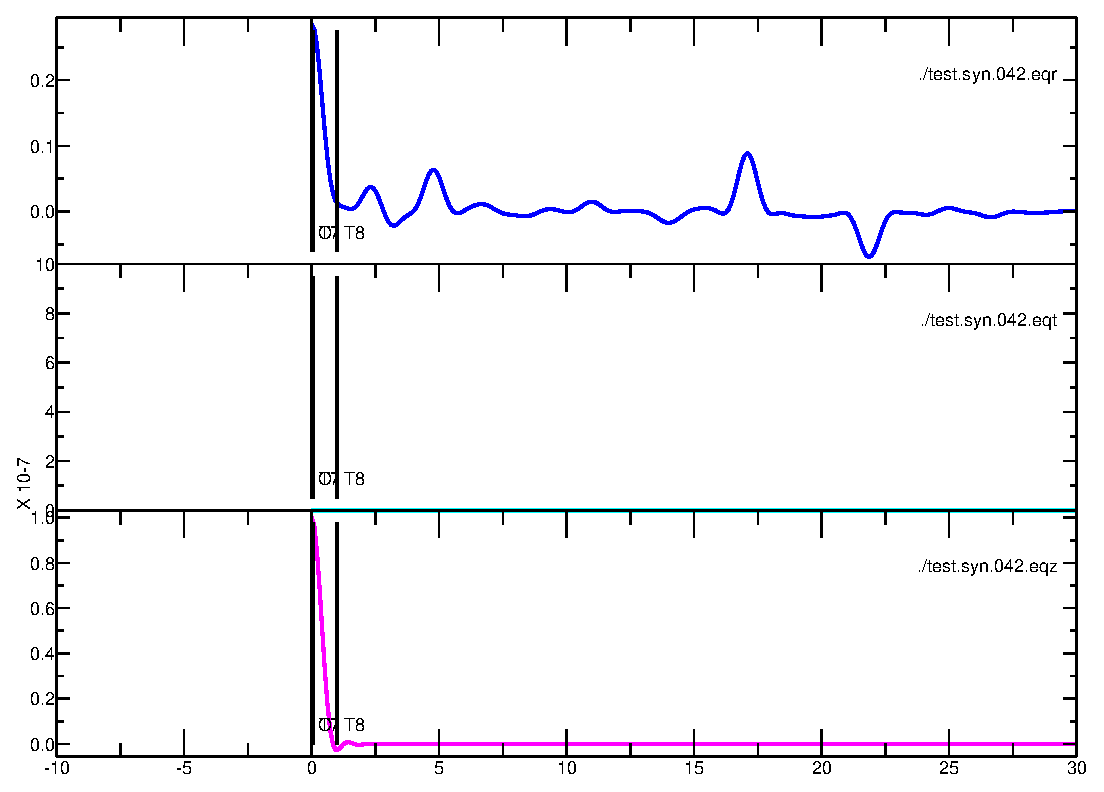
\includegraphics[width=13cm]{wave.eps}

\clearpage\section{反演}
这里介绍DERFmulti\_submit20090526\_v2包中的derfmod。其使用了差异演化算法()反演获得速度结构。terminal中的命令给出帮助信息:\par
\begin{bashCode}
bash> derfmod
***********************************************************
*Using DE method to search the best 1-D Model
*   (isotropic or anisotropic).
*Using Receiver Function waveforms in Z R T system.
*Only using R component in isotropic media.
*Using R and T components in anisotropic media.
***********************************************************
* derfmod  -Mmod -Bmod.scale -Drfs.list -Ggauss -Tbeg/end \
*	  [-Sst/seed/F/CR/NP/genmax] \
*         [-Ianiso -Hrfs.listT -WRweight/Tweight ]
*
* -M mod: 1-D model used to determine the searcing scales
* -B mod.scale 1-D searching scales relative to 1-D model
* -D rfs.list list of stacked RFs according ray parameter, 
       with stack number
* -G Gauss: Gauss filter for distrilling receiver functions
* -T beg/end: begin and end time relative to P onset for 
     inversion
*
* -I aniso: 0, Inverse for Isotropic Vp, Thickness, 
*              and Vp/Vs [0]
*	   -1, Inverse for Isotropic Vp, Thickness,
*              with fixed Vp/Vs
*	   -2, Inverse for Isotropic Vp, with fixed
*              Thickness and Vp/Vs
*	    1, Inverse for Anisotropic Model.
* -W weight: Rweight, weight for Radial RFs; 1>Rweight>0 
*	     Tweight, weight for tangential RFs;1>Tweight>0
*	     Rweight + Tweight = 1.0 
* -H rfs.listT list of stacked tangential RFs according ray 
               parameter, with stack number
* -S st: strategy for DE, can be 1 to 10.[3] integer
*    seed: random number seed,		 [5] integer
*    F: weight factor, 0<F<1,		 [0.85] float
*    CR: crossing over factor, 0<CR<1    [0.98] float
*    NP: population size, about 5-10 times of unknow para-
*        meters
*        [10] integer
*   genmax: maximum number of generations, [40] integer
\end{bashCode}
\par例子如下:\par
\begin{bashCode}
bash> derfmod -Messmod -Bessmod.DEB -Drfr.list \
      -G2.5 -T0.0/32.0 -I-1 -S3/5/0.85/0.98/10/50
\end{bashCode}
\par
命令参数中,-M指定了搜索中心模型文件,其文件格式与synrflzw中的essmod.syn相同;-B参数指定了一维搜索模型的范围,其文件内容格式是:\par
1.第1行是注释行;\par
2.第2行是半空间上的覆盖层数,这与搜索中心模型对应;\par
3.后续内容每2行指定了每一参数的搜索范围,参数顺序是:厚度,P波速,B,C,波速比,E,密度;\par
\begin{fileCode}
ESS forward model
4
0	0
5.0	0.6	0.0	0.0	0.0	0.0	0.0
0       0
5.0     0.6     0.0     0.0     0.0     0.0     0.0
0	0
5.0     0.6     0.0     0.0     0.0     0.0     0.0
0	0
10.0    0.6     0.0     0.0    	0.0     0.0     0.0
0	0
0.0     0.0 	0.0	0.0	0.0	0.0	0.0
\end{fileCode}
\par
-D参数指定了接受函数文件名list,本例子中,其内容如下。其中,第一列指定了文件名,第二列指定了此接收函数的叠加次数。\par
\begin{fileCode}
rfr/test.syn.056.eqr 1
\end{fileCode}
\par
-G参数指定了高斯滤波参数值;-T指定了时间序列截取的起始和终止相对时间;-I指定需要反演哪些参数,本例子中,反演各向同性介质中的层厚与P波速,这也与-B参数指定的模型参数搜索范围相对应;-W指定了径向与切向接收函数的权重,仅适用于各向异性反演;-H指定了切向接收函数的文件列表和叠加次数,其内容格式与-D参数相同,仅适用于各向异性反演;-S参数指定了差异演化算法的策略与对应的参数值。在例子中,选择策略3,随机数为5,权重因子未0.85,差异系数为0.98,每一代的人口数为10,演化代数为10。\par


\clearpage\section{基于KMI台的实验}
本小节以KMI台为例,从下载数据到接收函数提取,最后反演获得合理的速度模型。\par
\subsection{数据下载}
本例使用JWEED软件挑选台站与事件,下载事件文件。JWEED由IRIS提供,可以在http://ds.iris.edu/ds/nodes/dmc/software/downloads/jweed/下载。此软件有JAVA开发,可交互式挑选数据并下载。\par
本例选择KMI(昆明台)自2013-12-31-00:00:00~~2015-07-02-00:00:00,震中距30度~90度的内震级大于5.5的所有事件记录。时间截取长度选择P波出动前20s~后150s的数据。数据放在/home/wsh/JWEED.dir/Data\_KMI目录下。\par
\subsection{预处理数据}
使用JWEED下载的数据已经是SAC格式数据,其文件名格式是IC.KMI.00.BH1.M\_\_at\_\_2015-03-22T06.03.54.019Z.SAC,不可以直接用于XXX软件。更改后的文件格式是IC.KMI.00.M\_\_at\_\_2015-03-22T06.03.54.019Z.SAC.BH[NEZ],其中BH1对应BHN,BH2对应BHE。根据derfmod的需求,sac文件T7头段给定射线参数值。不需要其他预处理操作。\par
\subsection{提取接收函数}
使用pburg\_lzw做反褶积提取接收函数,pburg\_lzw的使用格式是:\par
\begin{bashCode}
bash> ../src/pburg_lzw <<EOF
2008.187.02.12.04
y
30
10
80
n
2.5
10
EOF
bash>
\end{bashCode}\par
其中,2008.187.02.12.04制定了文件名中除了后缀.BH[NEZ]的其他部分,y指定了地理坐标,30指定了B到A的时间差(s),10指定了截取A之前10s,80指定截取A之后80s,n指定不Taper,2.5是高斯参数,10指定接收函数结果延后10s。\par
使用脚本运行如下:\par
\begin{bashCode}
bash> decon.sh -D KMI/Data_KMI -L KMI/KMI.list.info \
      -R KMI/RFS -V
bash> #!Note:不要在-D参数后加"/"
bash> 
\end{bashCode}
\par
此脚本运行后,会在每一层子目录下生成相应接收函数,并在工作目录下生成KMI.list.info文件,其格式如下:\par
\begin{fileCode}
#Counts RF-PreName     Dir-Name
1 1.KMI.2015.03.2206 : 2015-03-22T05.56.22.3700_5.5
2 2.KMI.2015.03.2822 : 2015-03-28T22.28.50.7800_5.9
3 3.KMI.2015.03.2907 : 2015-03-29T07.50.54.2900_5.6
...
\end{fileCode}\par
\subsection{反演}
按照derfmod程序,要求,需要给定中心模型,及对应的搜索范围模型,以非线性搜索最合适的模型,在第7小节中给反演需要的不同的文件及其对应格式。本范例中,将由最简单的半无线空间单覆盖层开始,逐次增加模型的复杂度。\par
第一次反演,模型文件与模型搜索范围如下:\par
\begin{fileCode}
************** 1st Model  KMI.1.mod **************
Theta Phig
Thickness,Vp(km/s),B,C,Vp/Vs,E,density(g/cm^3),NSL
1
0 0
40.0    6.80    0.00     0.00   1.75    0.00    2.80    0
0 0
100.0	8.00	0.00	 0.00	1.80	0.00	3.30	0
\end{fileCode}
\par
\begin{fileCode}
************ 1st Model  KMI.1.mod.deb ************
1
0	0
10.0    0.5     0.0     0.0    	1.0     0.0     0.0
0	0
0.0     0.0 	0.0	0.0	0.0	0.0	0.0
\end{fileCode}

\end{CJK}
\end{document}
